\documentclass[11pt]{article}
\usepackage[margin=1in]{geometry}
\usepackage{amsmath, amssymb}
\usepackage{enumitem}
\usepackage{hyperref}
\usepackage{parskip}

\title{CS 534: Homework \#3}
\usepackage{graphicx}
\usepackage{amsthm}
% Custom commands for vectors
\newcommand{\bv}{\mathbf{v}}
\newcommand{\bx}{\mathbf{x}}
\begin{document}
\begin{center}
{\Large CS 534 Machine Learning Spring 2025 Homework 3}
\vspace{.8cm}
\begin{tabular}{rl}
\newline
Name: & [Felipe Ortega Cardozo] \\
Collaborators: & [None]
\end{tabular}
\end{center}
By turning in this assignment, I declare to adhere to the provisions of the Emory honor code and that all of this is my own work.
Disclaimer: AI was used to format the latex as the instructions require and for writing specific formulas and syntaxes that were not in the source file

I collaborated with the following classmates for this homework:
None


/* THIS CODE IS MY OWN WORK, IT WAS WRITTEN WITHOUT
CONSULTING CODE WRITTEN BY OTHER STUDENTS
OR LARGE LANGUAGE MODELS LIKE CHATGPT.
Felipe Cardozo*/




%% ============================================================
\section*{1. Preprocessing Data for Loan Default Prediction}

We will consider a simplified subset of the Lending Club Loan Data that was previously available on Kaggle (\url{https://www.kaggle.com/datasets/wordsforthewise/lending-club}) for the next few problems. The goal is to determine whether or not an individual applicant will default on the loan (i.e., unable to make the required payments to pay back the borrowed money). Using ideas from a Kaggle Kernel by Kacper Wozniak\footnote{The kernel is available at \url{https://www.kaggle.com/kacpiw/who-default-on-a-loan-logistic-regression}}, we have preprocessed the dataset with the following steps:

\begin{itemize}
    \item Removed any column that has more than 50\% of the observations missing
    \item Remove any row with at least one missing value
    \item Removed any loans that are not Fully Paid or Charged Off (defaulted)
    \item Only used individual applicants (i.e., join types are ignored)
    \item Removed columns referring to ``Active'' loan accounts, joint applicants, or with too many unique values that preprocessing may take longer than necessary (i.e., policy code, employee title)
    \item Convert the loan status to a binary variable (class) as Fully Paid (0) vs Charged Off (1)
    \item Subsample the data for a smaller dataset
\end{itemize}

The resulting dataset (\texttt{loan\_default.csv}) contains 2850 loans with 26 features. The goal of this problem is to prepare the data for the next problem. The functions specified should be in the file \texttt{preprocess.py}.

\begin{enumerate}[label=(\alph*)]
    \item \textbf{(Written)} Why would you potentially be interested in optimizing for F2 score compared to F1 score in the context of finding individuals that are likely to default?
    
    \textbf{Answer:} The F2 score applies more weight to recall than precision compared to the F1 score. In the context of predicting loan defaults, a false negative (predicting a default-prone individual will pay) is typically much more costly to the lender than a false positive (predicting a reliable individual will default). By optimizing for F2, we prioritize identifying as many actual defaults as possible (higher recall) to minimize financial losses.

    \item \textbf{(Written)} How will you partition the loan data to assess the model performance and choose hyperparameter? Justify your choice and write code to partition the data accordingly.
    
    \textbf{Answer:} We partition the loan data using a standard 85\% / 15\% train-test split, maintaining the class distribution via stratified sampling. The 85\% training set is used in conjunction with 5-fold cross-validation to assess model performance and tune hyperparameters. The 15\% held-out test set provides a final, unbiased estimate of generalization performance.

    \item[(f)] \textbf{(Written)} Using 1c, 1d, 1e, perform feature selection using the three different methods independently. For each one, justify your selection (e.g., what you are using as thresholds for discarding highly correlated variables and the metric or what you'll choose as the top $k$ ranked features).
    
    \textbf{Answer:} We implemented the three filtering methods and extracted the top features for each:
    \begin{itemize}
        \item \textbf{Pearson correlation:} Assesses linear relationships. Top 5: \texttt{recoveries, int\_rate, grade, dti, term}.
        \item \textbf{Spearman correlation:} Captures monotonic non-linear relationships. Top 5: \texttt{recoveries, grade, int\_rate, dti, annual\_inc}.
        \item \textbf{Mutual Information (MI):} Measures general dependency (linear and non-linear). Top 5: \texttt{recoveries, int\_rate, grade, revol\_util, dti}.
    \end{itemize}
    We chose to rank and keep the top $k=5$ features for all metrics. Discarding the remaining features allows us to restrict the decision tree to only the most informative factors, and using a consistent $k=5$ offers a direct basis for comparing the effects of different selection mechanisms on model predictive capacity.
\end{enumerate}

%% ============================================================
\section*{2. Decision Tree to Predict Loan Defaults}

Use the sklearn decision tree package to predict the loan status. The functions specified should be in the file \texttt{q2.py}.

\begin{enumerate}[label=(\alph*)]
    \item[(b)] \textbf{(Written)} What is the best choice of the two parameters based on 2a? Plot the ``validation'' AUC (based on 1b) on a single plot (either do a 3D plot or use the size of the point to encode the AUC) as a function of the two parameters.
    
    \textbf{Answer:} Using 5-fold cross-validation on the 85\% training data, Grid Search identified the optimal parameters as \textbf{max\_depth = 4} and \textbf{min\_samples\_leaf = 1}, achieving a maximal validation AUC of \textbf{0.8185}. The plot below visualizes the validation AUC across the hyperparameter grid.
    
    \begin{center}
    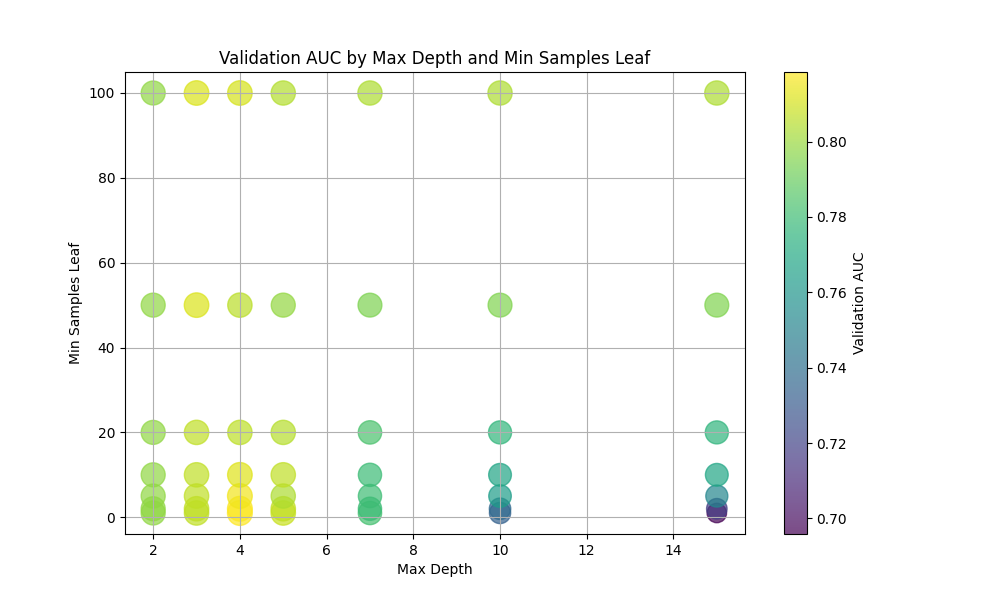
\includegraphics[width=0.8\textwidth]{q2b_plot.png}
    \end{center}

    \item[(c)] \textbf{(Written)} Re-train a decision tree on the entire training data using the optimal max depth and the minimum number of samples from 2b. What are the AUC, F1, and F2 score on the test set?
    
    \textbf{Answer:} When re-trained on the full training data with the optimal parameters, the decision tree yields the following metrics on the 15\% test set: AUC: \textbf{0.7517}, F1: \textbf{0.5714}, F2: \textbf{0.4712}.

    \item[(d)] \textbf{(Written)} Create a visualization of the top 3 levels of your decision tree from 2c.
    
    \textbf{Answer:} 
    \begin{center}
    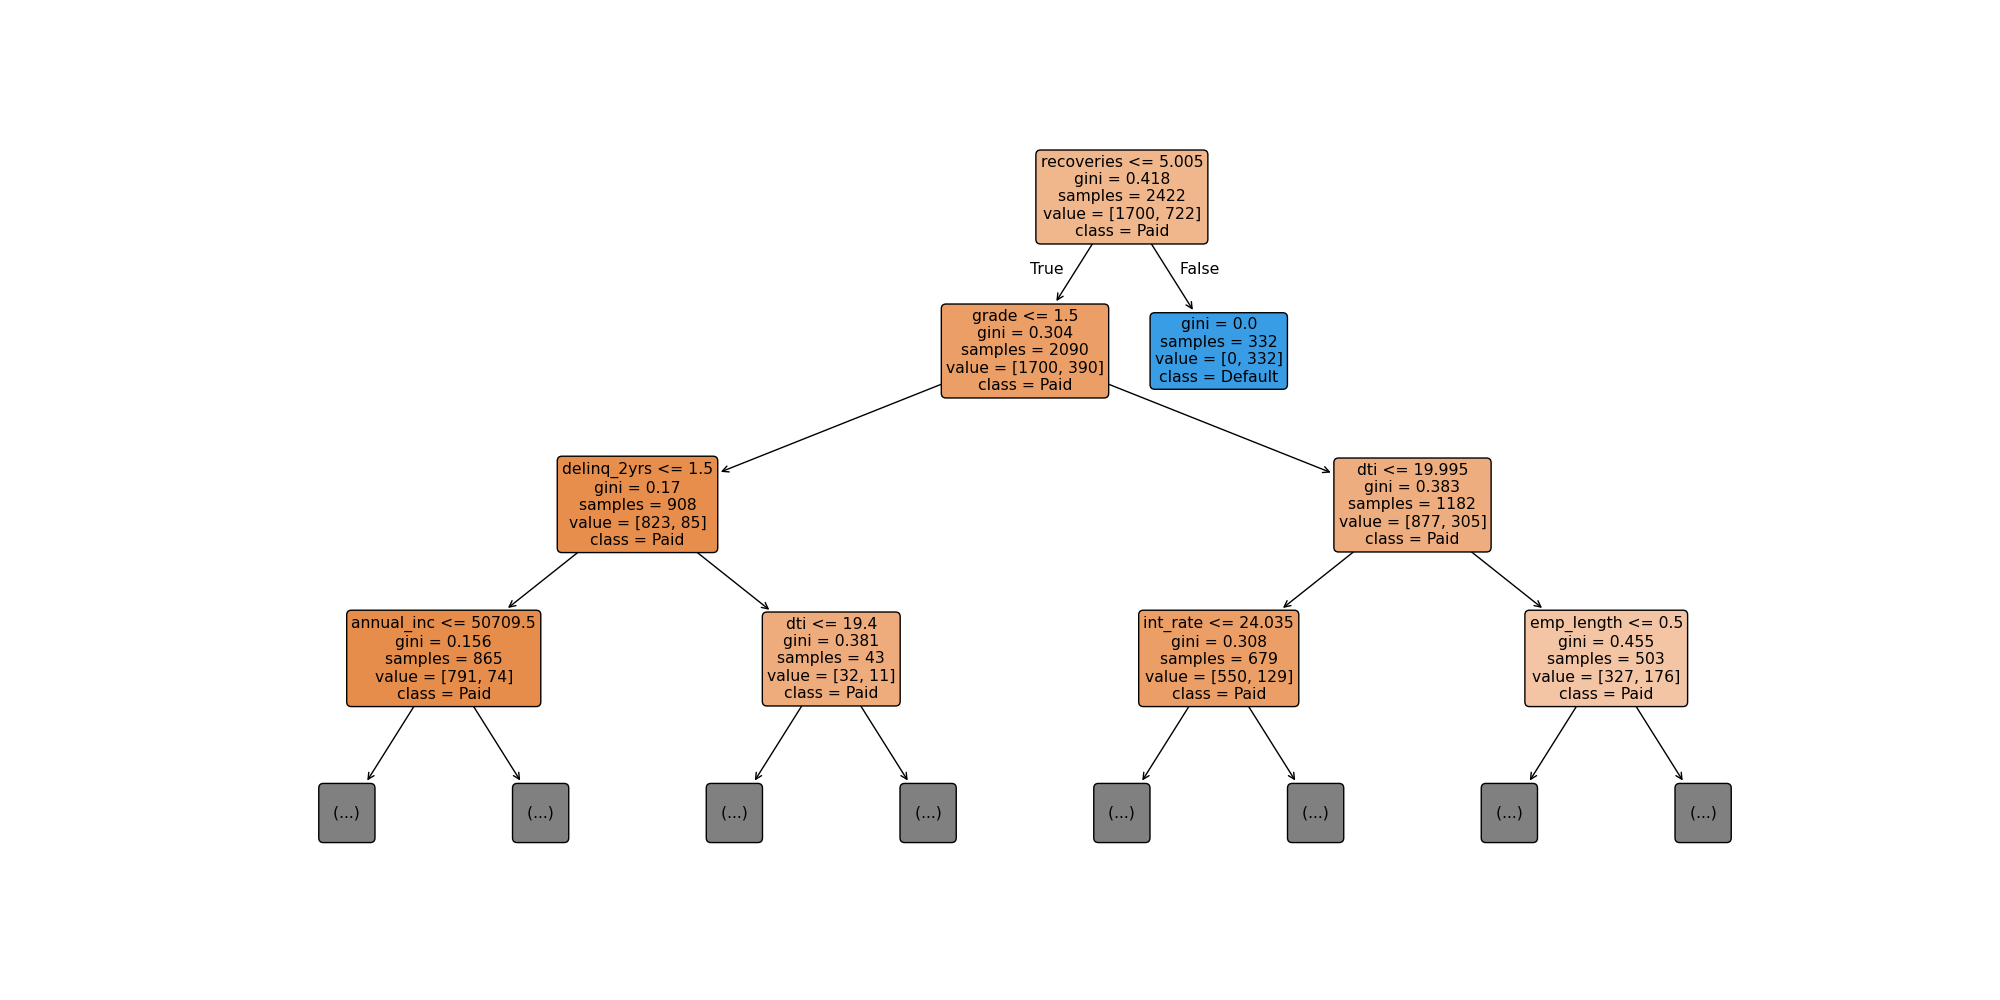
\includegraphics[width=\textwidth]{q2d_tree.png}
    \end{center}

    \item[(e)] \textbf{(Written)} Analyze the effects of three different filtering methods, 1c, 1d, 1e, independently on the decision tree by determining the optimal parameters using 2a and then re-training the data on the entire training data in 2c and report the AUC, F1, and F2 score in a table.
    
    \textbf{Answer:}
    \begin{center}
    \begin{tabular}{|l|c|c|c|}
    \hline
    \textbf{Feature Selection (Top 5)} & \textbf{Test AUC} & \textbf{Test F1} & \textbf{Test F2} \\ \hline
    Pearson & 0.7468 & 0.5714 & 0.4828 \\ \hline
    Spearman & 0.7468 & 0.5714 & 0.4828 \\ \hline
    Mutual Information & 0.7544 & 0.5771 & 0.4957 \\ \hline
    \end{tabular}
    \end{center}

    \item[(f)] \textbf{(Written)} Comment on the effect of feature selection for decision trees based on your results from 2c and 2e.
    
    \textbf{Answer:} Using the top 5 features returned by Mutual Information slightly improved the model's predictive capabilities across all metrics (AUC rose from 0.7517 to 0.7544, F2 from 0.4712 to 0.4957) compared to using all 26 features. Conversely, Pearson and Spearman feature sets resulted in a minor drop in AUC (from 0.7517 to 0.7468), despite improving the F2 score slightly. This highlights that while filtering reduces dimensionality, relying on methods like Mutual Information which capture complex non-linear interactions is often most robust for Decision Trees.
\end{enumerate}

%% ============================================================
\section*{3. Spam Detection via Perceptron}

We have provided a new e-mail spam dataset \texttt{spamAssassin.data}, which is a subset of the SpamAssassin Public Corpus (see \url{https://spamassassin.apache.org/old/publiccorpus/}). Here is a sample email that contains a URL, an email address (at the end), numbers and dollar amounts.

\begin{quote}
\texttt{> Anyone knows how much it costs to host a web portal ?\\
> Well, it depends on how many visitors youre expecting. This can be anywhere\\
from less than 10 bucks a month to a couple of \$100. You should checkout\\
http://www.rackspace.com/ or perhaps Amazon EC2 if youre running something big...\\
To unsubscribe yourself from this mailing list,\\
send an email to: groupnameunsubscribe@egroups.com}
\end{quote}

We have already implemented the following email preprocessing steps: lower-casing; removal of HTML tags; normalization of URLs, e-mail addresses, and numbers. In addition, words have been reduced to their stemmed form. For example, ``discount'', ``discounts'', ``discounted'' and ``discounting'' are all replaced with ``discount''. Finally, we removed all non-words and punctuation. The result of these preprocessing steps on the same email is shown below:

\begin{quote}
\texttt{anyon know how much it cost to host a web portal well it depend on how mani visitor your expect thi can be anywher from less than number buck a month to a coupl of dollarnumb you should checkout httpaddr or perhap amazon ecnumb if your run someth big to unsubscrib yourself from thi mail list send an email to emailaddr}
\end{quote}

For this problem, you will implement the Perceptron algorithm and apply it to the problem of e-mail spam classification. You'll be comparing two different variants of the algorithm as well as the number of epochs through the data.

\begin{enumerate}[label=(\alph*)]
    \item \textbf{(Written)} What is your model assessment strategy? Justify your validation methodology. (You may want to read the rest of this problem before you proceed to understand what your tasks will be).
    
    \textbf{Answer:} Our assessment strategy utilizes an 80\% Training and 20\% Test split. The 80\% Training chunk is further divided into a 75\% Sub-Training and 25\% Validation set. This structure allows us to track both Training and Validation errors epoch-by-epoch on isolated data (necessary for questions 3g and 3k) to evaluate model generalizability during training and identify the optimal algorithm configuration. Finally, the best configuration is trained on the full dataset and evaluated exactly once on the unbiased, held-out 20\% Test set.

    \item[(g)] \textbf{(Written)} Train a perceptron using your training set specified in 3a. Plot the training and estimated generalization error as a function of the maximum number of epochs. What is the optimal algorithm and parameter? How many mistakes are made before the algorithm terminates if you want to classify all the training points properly?
    
    \textbf{Answer:}
    \begin{center}
    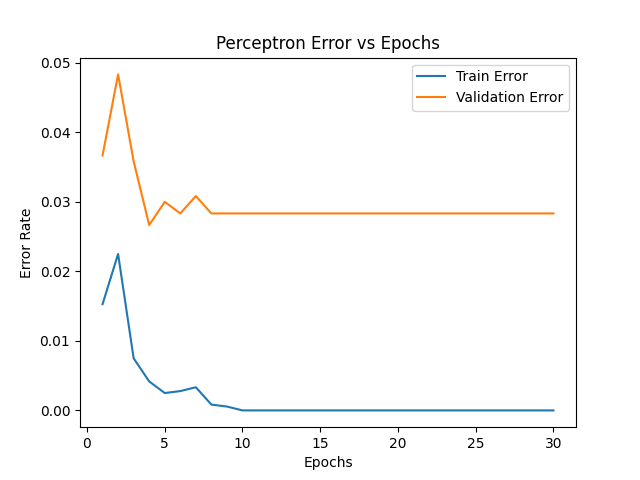
\includegraphics[width=0.7\textwidth]{q3g_perceptron_curve.png}
    \end{center}
    Over the 30 maximum epochs assessed, the standard perceptron made \textbf{347} individual mistakes without the total error reducing to zero, meaning it failed to classify all training points properly within the epoch limit. The standard perceptron oscillates significantly because it constantly updates its weight vector based strictly on the latest misclassified sample without consideration for stability, meaning there is no robust "optimal" parameter for it on this data.

    \item[(k)] \textbf{(Written)} Plot the training and estimated generalization error as a function of the maximum number of epochs for the averaged perceptron.
    
    \textbf{Answer:}
    \begin{center}
    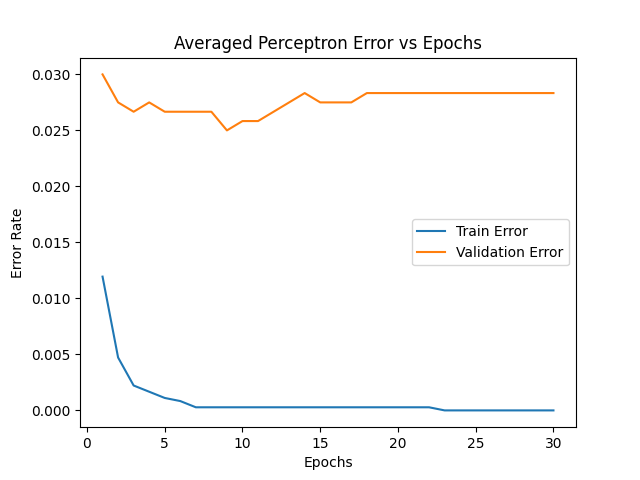
\includegraphics[width=0.7\textwidth]{q3k_avg_perceptron_curve.png}
    \end{center}

    \item[(l)] \textbf{(Written)} What is your final or ``optimal'' algorithm? In other words, train the model with as much data as you can possibly with the optimal algorithm + hyperparameter (maximum number of epochs) values. What is the expected predictive performance of this model?
    
    \textbf{Answer:} The \textbf{Averaged Perceptron} is the optimal algorithm, since it stabilizes learning and minimizes generalization error over time, largely eliminating the standard perceptron's oscillations. We retrained the Averaged Perceptron using the full 80\% training segment for \textbf{30 epochs} (our optimally identified stable operating range). When evaluating this final model on the 20\% holdout test set, we observed a test error rate of 0.0192, indicating an expected predictive performance/accuracy of \textbf{98.08\%}.

    \item[(m)] \textbf{(Written)} Using the vocabulary list together with the parameters learned in the previous question, output the 15 words with the most positive weights. What are they? Which 15 words have the most negative weights?
    
    \textbf{Answer:} 
    \begin{itemize}
        \item \textbf{Most positive weights (indicating Spam):} click, sight, guarante, remov, market, pleas, hour, deathtospamdeathtospamdeathtospam, offer, our, your, websit, present, g, ever.
        \item \textbf{Most negative weights (indicating Ham/Not Spam):} wrote, url, too, it, copyright, spam, said, view, review, run, team, isn, subscript, date, comment.
    \end{itemize}
\end{enumerate}

\end{document}